% Compile with XeLaTeX + BibTeX through latexmk. See README.md.
\documentclass[12pt,a4paper,oneside]{report}

% Editable document settings.
\newcommand{\DissertationTitle}{Integrating LiDAR and Machine Learning on Low-Cost ARM Microcontrollers for Autonomous Navigation}
\newcommand{\AuthorName}{TAO RAN}
\newcommand{\ProgrammeName}{Master of Science in Precision Scientific Instrumentation}
\newcommand{\SubmissionYear}{2026}

\usepackage[left=3.5cm,right=3cm,top=3cm,bottom=3cm]{geometry}
\usepackage{fontspec}
\IfFontExistsTF{Times New Roman}{
  \setmainfont{Times New Roman}
}{
  % Times-compatible preview font; use Times New Roman for submission.
  \setmainfont{texgyretermes-regular.otf}[
    BoldFont=texgyretermes-bold.otf,
    ItalicFont=texgyretermes-italic.otf,
    BoldItalicFont=texgyretermes-bolditalic.otf
  ]
  \PackageWarningNoLine{dissertation}{Times New Roman unavailable; using TeX Gyre Termes for this preview}
}
\usepackage{setspace}
% Paragraph style selected after checking SPMS theses in DR-NTU; see README.
% This is a house style, not a prescribed NTU indentation measurement.
\usepackage{indentfirst}
\setlength{\parindent}{1.27cm}
\setlength{\parskip}{0pt}
\usepackage{amsmath}
\usepackage{amssymb}
\usepackage{graphicx}
\usepackage{booktabs}
\usepackage{tabularx}
\usepackage{array}
\graphicspath{{figures/}{../experiment_data/}}
\newcommand{\mapname}[1]{\nolinkurl{#1}}
\usepackage[numbers,sort&compress]{natbib}
\usepackage[hidelinks]{hyperref}
\hypersetup{pdftitle={\DissertationTitle},pdfauthor={\AuthorName}}
\onehalfspacing
\setlength{\emergencystretch}{2em}
\clubpenalty=10000
\widowpenalty=10000
\setcounter{secnumdepth}{1}
\setcounter{tocdepth}{1}
\renewcommand{\contentsname}{Table of Contents}
\renewcommand{\bibname}{References}
\urlstyle{same}

\begin{document}
\hypersetup{pageanchor=false}

% Working draft. Official signed declarations will be added for submission.
\begin{titlepage}
  \centering
  \vspace*{1.5cm}
  {\Large\bfseries \DissertationTitle\par}
  \vspace{0.6cm}
  {\normalsize\itshape Digital-Twin-Oriented Training from an RL Teacher to Compact Navigation Policies\par}
  \vspace{1.4cm}
  {\large \AuthorName\par}
  \vfill
  {\normalsize SCHOOL OF PHYSICAL AND MATHEMATICAL SCIENCES\par}
  \vspace{1cm}
  {\normalsize A dissertation submitted in partial fulfilment of the requirements
  for the degree of\par}
  \vspace{0.4cm}
  {\normalsize \ProgrammeName\par}
  \vspace{1.2cm}
  {\large \SubmissionYear\par}
  \vspace{0.5cm}
  {\small Working draft: simulation study, 31 October 2026\par}
\end{titlepage}

\pagenumbering{roman}
\hypersetup{pageanchor=true}
\tableofcontents
\clearpage
% !TeX root = ../main.tex
\chapter*{Abstract}
\addcontentsline{toc}{chapter}{Abstract}
Training a compact navigation controller requires useful sensor--action examples,
which would otherwise need to be supplied by an operator or another expert.
This study investigates a digital-twin-oriented alternative: a virtual vehicle
learns to drive from reward feedback and then generates supervision for a
LiDAR-only controller intended for a resource-constrained, low-power development
board. Expensive learning and demonstration generation remain on the host;
the intended onboard workload is inference by the exported student.

The virtual training environment represents a differential-drive vehicle,
LiDAR and discrete steering interface in Gazebo. Proximal Policy Optimization
(PPO) trains a privileged neural teacher from geometric and vehicle-state
observations. The teacher uses separate multilayer-perceptron policy and value
branches, each with two 128-unit hidden layers. Its executed actions label
simultaneously paired LiDAR observations. Random forests are then fitted by
supervised behaviour cloning, using bounded-depth threshold tests and C++
export as the basis for later embedded integration. Thus RL learns the teacher;
it does not directly optimise the forest.

The original demonstration batch contains 1,439,983 scans and equally many
dropout copies, with three maps used for student fitting and one for validation.
Three 88-tree, depth-three forests and a single depth-six tree are evaluated
in 320 closed-loop episodes. The raw-only, combined-data and dropout-only forests
complete 67, 64 and 62 of 80 episodes, respectively; the single tree completes
74. All six single-tree failures occur under contiguous sector loss. A later
1,079,979-scan batch supports same-map offline assessment without retraining,
and host-side Python/C++ agreement checks pass on the tested inputs.

The results demonstrate automated supervision and useful compact-policy behaviour
in the tested simulation conditions. They also show that the initially selected
forest is not necessarily the strongest student configuration. Physical-twin
calibration, independent-map recovery, measured labour savings and target-board
memory, latency and energy remain unverified. The completed contribution is
the virtual training and policy-transfer stage of the proposed embedded workflow.

\clearpage
\phantomsection
\addcontentsline{toc}{chapter}{List of Figures}
\listoffigures
\clearpage
\phantomsection
\addcontentsline{toc}{chapter}{List of Tables}
\listoftables
\clearpage
\pagenumbering{arabic}

% !TeX root = ../main.tex
\chapter{Introduction}
\label{ch:introduction}
\section{Background and Motivation}
The purpose of this project is to develop a digital-twin-oriented training
workflow that replaces human driving demonstrations with automatically generated
supervision for a compact navigation policy. The intended outcome is a learned
LiDAR-to-steering controller that can ultimately run on a resource-constrained,
low-power development board. The central question concerns how such a controller
can be trained without requiring a person to drive and label every training
trajectory, while keeping the deployed computation small.

The intended vehicle uses a Teensy 4.0 ARM Cortex-M7 board~\cite{pjrcTeensy40}.
Training and deployment have different requirements: learning may use a host
computer, extensive simulation and information unavailable on the vehicle,
whereas onboard operation must process sensor data and produce commands within
memory, timing and energy budgets. Separating these stages permits a more capable
training system to produce a simpler deployed controller. Low-power operation
is an engineering objective of this separation; it is not an energy measurement
established by the present experiments.

In this dissertation, \emph{digital-twin-oriented training} denotes the use of
a parameterised virtual counterpart of the vehicle, sensor and control interface
to learn behaviour, generate demonstrations and test the resulting controller.
The implemented Gazebo model provides the virtual training side of this approach.
Physical calibration, live physical--virtual data exchange and experimental
confirmation of model fidelity remain future integration tasks. The present
study therefore evaluates the proposed training mechanism in simulation, without
assuming that a completed, continuously synchronised physical twin already exists.

The task is forward obstacle-avoiding cruising in static ring roads. Range-based
local control has classical precedents such as the Vector Field Histogram~\cite{borenstein1991vfh}.
Here, a learned policy converts fixed angular LiDAR bins into discrete steering
commands. The task provides a concrete setting in which to test automated
supervision and compact inference; route planning, SLAM and dynamic traffic are
outside the evaluated scope.

\section{Problem Statement}
A supervised random-forest controller needs examples of what action to take
for each sensor observation. Under a human-demonstration approach, an operator
must drive the vehicle while observations and commands are recorded. Covering
new roads, starting conditions and sensor conditions can require further
collection. Merely choosing a compact classifier does not solve this source-of-labels
problem: the fitting algorithm still needs informative, correctly paired examples.

The virtual vehicle offers a different route. Its simulated interaction provides
travel, clearance and collision feedback from which a policy can learn without
pre-existing steering labels. Once learned, that policy can drive the simulated
vehicle and supply labels automatically. Reinforcement learning (RL) is therefore
used to obtain a \emph{teacher}, rather than to perform the final random-forest
fitting directly. In the implemented workflow, Proximal Policy Optimization
(PPO) trains a neural teacher~\cite{schulman2017ppo}; supervised behaviour cloning
then fits the random forest to the teacher's LiDAR--action pairs.

This arrangement must solve three connected engineering problems. First, reward
and termination definitions must produce a teacher whose behaviour is useful
for the driving task. Second, scan and action records must preserve the
observation--decision relationship, because an incorrect temporal pairing would
create misleading supervision even for a capable teacher. Third, the student's
restricted input and model capacity must retain useful behaviour when it drives
on its own. Teacher performance does not guarantee student performance: the
student can change its future observations through its own errors~\cite{ross2011reduction}.

Replacing human demonstrations does not eliminate human engineering. Vehicle
modelling, reward design, scenario selection and acceptance criteria remain
human decisions. The completed experiments establish automated collection of
action labels; they do not quantify labour savings or establish superiority over
a human-trained controller, since no matched human-demonstration study has been
performed.

\section{Proposed Approach and Method Rationale}
The proposed solution separates learning to drive from learning a deployable
sensor-to-action mapping. A privileged teacher first learns in simulation using
map-derived distances and vehicle state. During demonstration collection, the
same simulated vehicle produces LiDAR scans and executes teacher actions. A
student then learns from these paired observations and commands, and is evaluated
in closed loop using LiDAR alone. This information separation is related to
privileged-to-sensor policy transfer~\cite{chen2019cheating}.

RL is selected because it can optimise behaviour from the consequences of
sequential actions without first requiring a labelled driving dataset. PPO is
the specific training algorithm: its clipped policy update and established
actor--critic implementation provide a practical way to train from simulated
rollouts~\cite{schulman2017ppo,raffin2021sb3}. The teacher model is a feed-forward
multilayer perceptron (MLP), with separate policy and value branches. PPO is thus
an optimisation method, MLP is the teacher's function approximator, and random
forest is the separately fitted student model. These terms describe different
parts of the workflow.

Random forests are selected as the principal student family because numerical
LiDAR bins can be partitioned by threshold tests, and tree depth and tree count
provide explicit controls over inference work~\cite{breiman2001random,sklearnForest}.
The fitted decision structures can be exported to C++ without running a neural
training framework on the vehicle. An ensemble also offers a way to combine
several partitions instead of relying on one tree. These are design motivations,
not guarantees of minimal memory, lowest power or best navigation performance.
A deeper single tree is included to test whether the ensemble's extra structure
is justified by the observed results.

The rationale is consequently a division of responsibilities: simulation supplies
repeatable interaction, RL supplies a teacher without human action labels,
behaviour cloning transfers its commands to sensor inputs, and tree inference
provides a controllable implementation for later embedded integration. Alternative
teachers and compact student families remain possible; this study evaluates one
concrete, reproducible route rather than claiming that each choice is universally
optimal.

\section{Objectives and Research Questions}
The overall objective is to demonstrate an automated path from a virtual vehicle
to a compact navigation policy, with evidence at each transition. The specific
objectives are to train and qualify an RL teacher, generate traceable demonstrations,
fit LiDAR-only students, assess the transfer of useful behaviour, and verify
exported inference before eventual board deployment.

Three questions organise the investigation:
\begin{description}
\item[RQ1: Automated supervision.] Can an RL teacher generate useful paired
LiDAR--action demonstrations in the virtual vehicle without human driving
labels, and can that collection be repeated with documented provenance?
\item[RQ2: Transfer to compact policies.] Can random-forest students retain
useful closed-loop behaviour from these demonstrations, how do they compare
with a single-tree baseline, and what limits appear under sensor loss?
\item[RQ3: Resource-constrained deployment.] Why is the selected tree
representation suitable for pursuing embedded inference, what does the verified
export establish, and which resource and physical measurements remain necessary?
\end{description}

The first question is examined through teacher qualification and two recorded
collection batches. The second uses offline prediction, primary closed-loop
comparisons and repeat runs. The third is addressed through model structure,
interface compatibility and host-side C++ agreement; actual board-level
performance remains an open experimental part of the project.

\section{Scope and Contributions}
The completed contribution is an integrated training workflow, not a new RL
algorithm or tree-learning rule. It links a parameterised virtual vehicle, a
privileged PPO teacher, automated demonstration collection, map-separated
student fitting and closed-loop evaluation. Model, map and episode records make
the supervision source traceable, and export checks connect fitted predictions
to executable C++ inference.

The primary comparison comprises 320 episodes across four controller
configurations. The single depth-six tree completes 74 of its 80 episodes,
whereas the three shallow forests complete between 62 and 67. This finding
supports evaluating the simplest useful student instead of treating a random
forest as a required winner. It also identifies a limit of the training approach:
every candidate experiences collisions under contiguous sector loss. The
comparison is configuration-specific because depth, sampling and ensemble size
are not all held constant.

Three maps supply student fitting data, while \mapname{ellipse_002} is used for
validation and selection. It is therefore not an untouched final test map~\cite{sklearnCV}.
A later batch tests consistency on the same map set without retraining. Independent-map
recovery, target-board resource consumption, physical driving and physical--virtual
fidelity have not yet been measured. The observed simulation results support the
training mechanism while leaving these broader deployment questions open.

\section{Organisation of the Dissertation}
Chapter~\ref{ch:literature} places the training strategy and compact policies in
context. Chapter~\ref{ch:system} describes the virtual counterpart and interfaces.
Chapter~\ref{ch:teacher} explains the RL choice, teacher architecture and automated
collection. Chapter~\ref{ch:student} develops the random-forest rationale, fitting
and export. Chapter~\ref{ch:results} evaluates the resulting workflow and its
limits. Chapter~\ref{ch:conclusions} answers the research questions and identifies
the remaining work. Appendix~\ref{app:evidence} records the principal evidence
sources.

% !TeX root = ../main.tex
\chapter{Literature Review}
\label{ch:literature}
\section{Training Strategy and Deployment Objective}
The methodological background is organised around the project's separation of
training and deployment. A virtual vehicle supplies interaction, RL learns a
teacher, imitation creates a sensor-limited student, and a compact model provides
the candidate for board inference. The objective is to replace manually supplied
driving examples while retaining useful behaviour in a constrained implementation.
The subsequent model comparison evaluates this training strategy rather than
introducing a new tree or policy-gradient algorithm.

Kritzinger et al. distinguish digital models, digital shadows and digital twins
according to their level of integration~\cite{kritzinger2018digital}. This
distinction prevents a simulator from being treated as evidence of a fully
connected physical--digital system. In this dissertation, the virtual vehicle
implements the training side of an intended digital-twin workflow; measured
physical calibration and synchronisation are still required.

The digital-twin-oriented scope is operationally defined in
Chapter~\ref{ch:introduction}: a vehicle-specific virtual counterpart supports
learning and collection, while calibration and physical coupling remain pending.
The cited simulation platform supplies the enabling environment~\cite{koenig2004gazebo};
its existence alone does not establish physical fidelity for this vehicle.
Likewise, privileged-policy transfer motivates the separation of teacher and
student information~\cite{chen2019cheating}, but provides no substitute for
measuring the present student's behaviour.

\section{Local Feedback Control}
The engineering question in this study concerns a local feedback controller:
a range observation is converted into a steering decision, which changes the
next observation. This differs from evaluating a classifier on an independent
collection of labelled samples. It also differs from global navigation, where
route choice and destination progress require additional task definitions.
The literature considered here is selected to explain teacher learning,
student imitation, tree-based inference and simulation perturbations.

A classical example is the Vector Field Histogram (VFH) of Borenstein and
Koren~\cite{borenstein1991vfh}. It maintains a Cartesian obstacle histogram
and derives a polar representation from which a steering direction is selected.
The present student instead maps a single binned scan directly to an action
learned from demonstrations. Both approaches use directional range information,
but the student does not implement VFH's obstacle grid or selection rule.
VFH is methodological context here; no experimental comparison with VFH has
been conducted.

Tai, Paolo and Liu demonstrate a different route to obtaining navigation
behaviour without prior driving demonstrations: a deep RL policy maps ten range
measurements and a relative target position to continuous steering commands,
with reported tests in virtual and real environments~\cite{tai2017virtual}.
This supports investigating simulation interaction as a source of behaviour.
Their goal-directed neural controller differs from the present forward-cruising,
discrete-action task. Here the learned teacher supplies examples for a separate
tree student, and the reported evidence remains simulation-only. Their physical
transfer results cannot be attributed to the present vehicle.

For the present vehicle, the sensor representation is part of the control
design. Discretising distance by angle fixes the relationship between input
columns and physical directions. Suppressing the rear sector reduces available
information, while using zero for missing returns makes missingness a feature
of the learned policy. A comparison of learning algorithms is meaningful only
when these conventions and the action interface remain explicit.

\section{Random Forests and Compact Tree Policies}
Breiman introduced random forests as ensembles of randomised tree predictors
and analysed their generalisation behaviour in relation to the strength and
dependence of individual trees~\cite{breiman2001random}. The relevant design
idea is that multiple trees can provide different partitions of the input
space. An ensemble nevertheless requires more inference work than a single
tree, and its performance depends on how those partitions are constructed.

In this project, depth and tree count are explicit model choices. A shallow
forest permits several small decision structures to contribute to a prediction;
a deeper single tree permits a longer sequence of conditional decisions along
one path. These are different ways of allocating capacity. Neither allocation
can be declared superior for the vehicle without checking the states reached
during closed-loop operation.

The implementation uses scikit-learn 1.7.2, from the machine-learning library
described by Pedregosa et al.~\cite{pedregosa2011sklearn}. Its random-forest classifier
aggregates class probabilities from the trees, with bootstrap sampling and
random feature selection available during fitting~\cite{sklearnForest}.
This detail matters when exporting inference: replacing probability averaging
with hard majority voting would define a different controller. The study
therefore verifies agreement after export rather than treating any generated
C++ tree code as automatically equivalent.

Embedded tree learning also has more specialised alternatives. Kumar, Goyal
and Varma's Bonsai jointly learns a sparse projection and a shallow tree with
expressive nodes, targeting devices with as little as 2~KB of
RAM~\cite{kumar2017bonsai}. Its design shows why resource constraints should
affect model construction, rather than being checked only after fitting.
Bonsai is not an ordinary random forest, and its published memory results do
not describe the exported models in this project. The present forest provides
a simpler existing fitting/export path; the single-tree comparison tests
whether that ensemble complexity is justified by the observed behaviour.

Nor are trees the only feasible microcontroller models. Lai, Suda and Chandra
develop CMSIS-NN kernels to improve neural inference efficiency on Arm Cortex-M
CPUs~\cite{lai2018cmsis}. Thus a compact neural student is a credible alternative,
especially on a Cortex-M7 with floating-point support. Selecting a forest here
rests on its threshold representation, bounded traversal and verified C++ export,
not on an assertion that neural networks cannot execute on the target board.
An equal-budget neural comparison remains future work.

\section{Learning a Privileged Teacher}
PPO uses a policy-gradient objective with a clipped probability ratio to
moderate updates relative to the data-collecting policy~\cite{schulman2017ppo}.
Here it supplies the teacher policy rather than the final tree model. A neural
policy can use the simulated distance field and vehicle state while generating
examples for a more restricted student.

The separation of a privileged policy from a sensor-limited policy is related
to the two-stage approach in \emph{Learning by Cheating}. Chen et al. first
learn a policy with privileged information and then transfer behaviour to an
agent using ordinary observations in a driving simulator~\cite{chen2019cheating}.
The present project differs in its small differential-drive platform, LiDAR
bins, discrete steering labels and tree-based student. The cited work motivates
the information separation; it does not validate the present implementation.

A privileged teacher should not be interpreted as an available physical
controller. Its geometry is supplied by the simulator, and the student does
not acquire that geometry merely by imitating actions. Evaluating teacher and
student as if they had identical information would conceal a central design
constraint.

Rusu et al. show that an RL policy can be transferred to a smaller neural
network through policy distillation~\cite{rusu2015distillation}. Bastani, Pu and
Solar-Lezama's VIPER instead extracts a decision-tree policy from a neural
oracle using its Q-function, enabling verification in their benchmark
settings~\cite{bastani2018viper}. Together these works motivate separating the
model that learns the task from the model chosen for deployment. The present
pipeline uses hard action labels and ordinary supervised fitting; it does not
implement VIPER's Q-guided extraction or establish its formal guarantees.
The match to the research objective is the teacher--student separation, while
the collection procedure and validation claims remain specific to this project.

\section{Behaviour Cloning and Distribution Shift}
Ross, Gordon and Bagnell show why sequential prediction differs from ordinary
independent supervised prediction: actions influence future observations.
Their DAgger approach collects expert-labelled examples on states encountered
by the learner~\cite{ross2011reduction}. The distinction is relevant when
interpreting a student that performs well on teacher scans but fails after its
own steering changes the trajectory.

The present pipeline performs behaviour cloning on teacher-driven episodes.
Perturbed and near-wall teacher starts expand the demonstration conditions,
but there is no iterative learner-execution and expert-relabeling loop.
Consequently, the implementation is not described as DAgger. Likewise, labels
are discrete teacher commands, not teacher probability distributions; no
soft-label distillation loss is used.

This methodological boundary leads to a practical evaluation requirement.
Prediction disagreement is measured offline, but collisions and recovery
must be measured while the student actually drives. High agreement on common
straight-driving examples cannot establish adequate behaviour in a rare
turning state or after a loss of sensor coverage.

\section{Simulation Perturbations and Transfer}
Tobin et al. investigate domain randomisation by varying rendered simulation
conditions to support transfer of vision-based learning to physical
robotics~\cite{tobin2017domain}. That work establishes a motivation for varying
training conditions, but its image-based transfer result is not evidence that
any particular LiDAR corruption will improve the controller studied here.

The present experiments distinguish scattered point loss from contiguous
sector loss. These perturbations remove information in different spatial
patterns. A training procedure that masks a small number of separated
measurements need not provide examples of an extended blind region. The
experimental question is therefore whether the chosen augmentation matches
useful deployment variation, not simply whether augmented data are present.

Simulation also provides exact state and an idealised velocity interface.
Physical transfer would introduce sensor calibration, command-response and
timing questions. Those measurements are outside this draft, so simulation
robustness is discussed within the implemented perturbation families.

\section{Positioning of the Study}
Table~\ref{tab:literature} connects the selected methodological sources to the
choices made in this project. This is a focused initial review, not a claim
that these sources exhaust LiDAR navigation or embedded machine learning.
The contribution is the experimentally traceable combination of established
methods under a common observation, action and evaluation contract.

\begin{table}[htbp]
\centering\small
\caption{Methodological context and its role in this study.}
\label{tab:literature}
\begin{tabularx}{\textwidth}{p{3.1cm}>{\raggedright\arraybackslash}X>{\raggedright\arraybackslash}X}
\toprule
Source & Relevant idea & Boundary in this study \\
\midrule
Breiman~\cite{breiman2001random} & Randomised tree ensembles & Forest superiority is tested, not assumed. \\
Schulman et al.~\cite{schulman2017ppo} & Clipped policy optimisation & PPO trains the privileged teacher. \\
Chen et al.~\cite{chen2019cheating} & Privileged-to-sensor policy transfer & Student and task differ from the cited driving system. \\
Ross et al.~\cite{ross2011reduction} & Learner-induced state distribution & No iterative DAgger collection is implemented. \\
Tobin et al.~\cite{tobin2017domain} & Training-condition variation & LiDAR masking is assessed separately from physical transfer. \\
\bottomrule
\end{tabularx}
\end{table}

The reviewed work leads to a coherent selection: simulation supplies repeated
interaction; PPO provides the neural teacher; behaviour cloning transfers
actions to the LiDAR interface; and bounded-depth trees expose a manageable
inference structure. Each selection addresses a different constraint. The
literature motivates this combination but does not establish that it is the
best-performing or lowest-power combination for the vehicle.

The empirical gap addressed by the experiments is narrow and concrete:
whether automatically generated teacher demonstrations produce useful compact
students, and whether the initially selected forest retains its appeal when
offline agreement and closed-loop behaviour are assessed separately. A broader survey of
microcontroller navigation systems and directly comparable physical platforms
remains appropriate for the final dissertation, when the hardware scope and
measurements are settled.

% !TeX root = ../main.tex
\chapter{Virtual Vehicle and Digital-Twin Training Workflow}
\label{ch:system}
\section{Virtual Counterpart and Training Scope}
The virtual counterpart represents the vehicle geometry, differential-drive
motion, LiDAR configuration, command labels and task environment needed for
training. Shared parameters make these assumptions explicit and reproducible.
For example, wheel radius and separation determine the kinematic conversion,
while scan layout and distance units determine the student's input contract.
This coupling is the practical reason for using a vehicle-specific virtual
model instead of generating arbitrary range vectors with invented labels.

The role of this counterpart is to support interaction that would otherwise
require repeated driving of the physical vehicle. It can reset starts, expose
map geometry to the teacher and collect sensor/action pairs over long runs.
These capabilities support the intended digital-twin workflow. They do not
show that simulated friction, range noise or motor response have been fitted
to physical measurements. The present model is a parameterised training
representation, with physical fidelity and synchronisation still to be assessed.

The legacy physical firmware also uses different steering and timing conventions.
Consequently, the common simulation interface is not yet a demonstrated
end-to-end physical interface. The next integration stage must reconcile
those conventions and validate the virtual model against the actual vehicle.

\section{Training and Deployment Architecture}
The implementation combines ROS~2 communication~\cite{macenski2022ros2}
with Gazebo Classic physics, using the simulation framework introduced by
Koenig and Howard~\cite{koenig2004gazebo}.
A shared vehicle configuration defines geometry, sensor settings and steering
labels. Teacher training, demonstration collection and student evaluation use
these definitions, while saved run configurations provide the historical
settings for individual experiments. Current source defaults are not used as
substitutes for the configuration stored with an older model.

The learning sequence is shown in Figure~\ref{fig:pipeline}. During teacher
operation, map geometry and vehicle state enter the learned neural policy,
which selects an action. Collection
also records LiDAR, but LiDAR does not become an input to that privileged
policy. During student evaluation, the policy receives LiDAR only; geometry
and state remain available to the evaluator for scoring.

\begin{figure}[htbp]
\centering
\fbox{\parbox{0.89\textwidth}{\centering
\textbf{Virtual training on the host}\\[5pt]
Vehicle, sensor and task model $\longrightarrow$ simulated interaction\\[5pt]
Reward feedback $\longrightarrow$ PPO training of an MLP teacher\\[5pt]
Teacher commands + paired LiDAR $\longrightarrow$ labelled dataset\\[5pt]
Supervised fitting $\longrightarrow$ random forest / single tree\\[5pt]
Student closed-loop evaluation + C++ agreement checks\\[8pt]
$\downarrow$\\[5pt]
\textbf{Intended onboard inference}\\[5pt]
Physical LiDAR $\longrightarrow$ exported student $\longrightarrow$ motors\\[3pt]
Physical calibration and board validation remain pending}}
\caption[Teacher-to-student information flow]{Implemented information flow. Geometry used by the evaluator does
not enter the student's feature vector. The lower stage is the intended
physical integration path, not a completed experiment.}
\label{fig:pipeline}
\end{figure}

This separation avoids evaluating a purported LiDAR controller that silently
uses ground-truth distances. It also enables geometric clearance to be
computed independently of sensor corruption. A missing scan can affect the
policy without simultaneously hiding an obstacle from the scoring system.

\section{Differential-Drive Action Interface}
Let $a\in\{0,\ldots,14\}$ be a steering label, with $a=7$ denoting straight
motion. The implemented targets are
\begin{align}
 s(a)&=\frac{7-a}{7}, & \Delta v(a)&=\rho v_0 s(a),\\
 v_L(a)&=v_0-\Delta v(a), & v_R(a)&=v_0+\Delta v(a),
\end{align}
where $v_0=0.2\,\mathrm{m\,s^{-1}}$ and $\rho=0.6$. With wheel separation
$b=0.11\,\mathrm{m}$, the ideal differential-drive relation~\cite[Chapter~13]{lynch2017modern} gives
\begin{equation}
 v=\frac{v_R+v_L}{2}=v_0,\qquad
 \omega=\frac{v_R-v_L}{b}.
\end{equation}
Wheel angular targets are obtained by division by the configured radius
$r=0.0325\,\mathrm{m}$. At the strongest steering commands the linear wheel
targets are $0.08$ and $0.32\,\mathrm{m\,s^{-1}}$. Thus all ordinary steering
actions continue forward. An ideal maximum-curvature radius computed from
these targets is about $0.092\,\mathrm{m}$; actual collision-free passage also
depends on body dimensions, wall shape and the finite control interval.

The stop command is a separate interface value, 200, and is not a learned
steering class. The model therefore selects curvature at an approximately
fixed centre speed, rather than jointly optimising forward speed and turning.
This restriction limits the conclusions to roads that can be traversed with
forward-only control.

\section{LiDAR Representation and Missing Values}
Raw scan angles are first converted to integer degrees. For an angle $\theta$
in degrees, the feature index is
\begin{equation}
 i=\left\lfloor\frac{200\lfloor\theta\rfloor}{360}\right\rfloor,
 \qquad 0\leq\theta<360.
\end{equation}
Distances are represented in integer millimetres. Values outside the accepted
positive range below 10,000~mm are represented as invalid rather than extended
to arbitrary large measurements. The physical sensor range in the simulator
and the feature representation limit are distinct settings.

The active indices are $0$--$49$ and $151$--$199$. The remaining 101 indices
are fixed zero, leaving 99 active angular bins. Zero in an active bin denotes
a missing or unusable reading. A model trained on these inputs must therefore
interpret both angle and missingness consistently. Removing all rows containing
a zero would incorrectly discard valid scans because the inactive sector is
always zero.

Table~\ref{tab:platform} gives the settings used for the reported collections
and student evaluations. The 1~cm noise standard deviation is a simulation
assumption, not a measured calibration error. Earlier teacher configurations
recorded a different raw ray count, but the teacher did not use LiDAR; the
student dataset and evaluated sensor configuration use 364 rays per revolution.

\begin{table}[htbp]
\centering\small
\caption{Principal simulation settings for the student experiments.}
\label{tab:platform}
\begin{tabularx}{\textwidth}{Xl}
\toprule Parameter & Value \\\midrule
Target forward speed & $0.2\,\mathrm{m\,s^{-1}}$ \\
Wheel radius / separation & $0.0325/0.11\,\mathrm{m}$ \\
Steering labels / straight label & $0$--$14$ / $7$ \\
Decision interval / physics step & $0.2/0.001\,\mathrm{s}$ \\
LiDAR scan rate / raw rays & $5.5\,\mathrm{Hz}$ / $364$ \\
LiDAR physical range & $0.15$--$12\,\mathrm{m}$ \\
Feature distance upper limit & $10\,\mathrm{m}$, exclusive \\
Range-noise standard deviation & $0.01\,\mathrm{m}$ \\
Input columns / active bins & $200/99$ \\
Conservative body radius for clearance & $0.085\,\mathrm{m}$ \\
\bottomrule
\end{tabularx}
\end{table}

\section{Maps and Experimental Roles}
Four static ring roads are used: \mapname{train_world3},
\mapname{rounded_rectangle_001}, \mapname{rounded_rectangle_003} and
\mapname{ellipse_002}. For compact tables, these are denoted T3, R1, R3 and
E2, respectively. Wall geometry is represented by static obstacles, and
same-stem map metadata provide spawn poses and workspace bounds.

The selected teacher was trained and qualified on T3. It subsequently supplied
demonstrations on all four maps. Student fitting uses T3, R1 and R3; E2 is
withheld from fitting but used for validation and selection. The distinction
between teacher training, teacher collection, student fitting and student
selection prevents an ambiguous claim that a map is simply ``unseen''.
Figure~\ref{fig:collisionmaps} later shows the four geometries with recorded
collision endpoints.

\section{Timing and Evaluation Boundaries}
The formal closed-loop evaluator pauses Gazebo between controlled steps and
uses a nominal 0.2~s simulation decision interval. This supports repeatable
state/action records, but does not demonstrate wall-clock real-time operation.
The GUI driver operates asynchronously and is not the source of the formal
comparison matrices.

Scoring uses a conservative body disc and map-derived obstacle distance.
Clearance is sampled at decision steps, so its minimum is a sampled geometric
measure. Contact-based collision detection is a different signal. A reported
zero clearance can therefore occur without a recorded collision; neither
quantity should silently replace the other.

The intended hardware implementation must eventually reproduce the input and
action contract. The legacy firmware uses different steering and timing
conventions, so no physical equivalence is assumed here. All numerical results
in the following chapters concern the saved simulation configurations.

% !TeX root = ../main.tex
\chapter{Reinforcement-Learning Teacher and Automated Demonstrations}
\label{ch:teacher}
\section{Why Reinforcement Learning Is Used}
The teacher is needed because the student requires action labels and the
proposed workflow seeks to obtain them without manual driving demonstrations.
RL supplies a mechanism for learning a policy from simulated interaction:
steering changes the trajectory, and reward feedback evaluates the subsequent
motion. Forward travel, clearance and collision outcomes can be computed by
the virtual environment without an operator specifying an action for every
scan. The resulting teacher can then generate the supervised dataset.

The distinction between reward design and action labelling is central. A reward
states what outcomes are desirable; it does not enumerate the steering command
for every encountered state. RL is useful here because a locally plausible turn
can affect later collision risk, so the training objective must consider a
sequence of decisions. This does not remove the need to design suitable rewards
or to qualify the teacher before collecting its demonstrations.

A manually programmed expert or a classical planner could also generate labels.
Such a teacher would require an explicit control strategy and appropriate
vehicle/task assumptions. The present project selects RL to learn that strategy
from interaction. It has not compared the cost or quality of all possible
teacher sources, and it does not claim that RL is the only route to automated
supervision.

\section{Why PPO Is Selected}
PPO is an on-policy actor--critic algorithm that updates a policy using recently
collected rollouts. Its clipped surrogate limits the incentive for some large
probability-ratio changes, providing a practical update mechanism without
requiring gradients through the simulator~\cite{schulman2017ppo}. The chosen
implementation provides the policy, value estimation and rollout machinery
within a consistent training interface~\cite{raffin2021sb3}.

These properties suit this workflow: the simulator can repeatedly reset and
execute the fifteen-action interface, while the host performs optimisation.
The selected run uses four parallel environments and 512 rollout steps per
environment before an update. PPO is an engineering choice supported by the
available implementation and observed teacher qualification, not a demonstrated
winner over every RL algorithm. On-policy learning also requires new interaction
after updates, so its simulation cost remains part of the training cost.
No algorithm-comparison experiment establishes that PPO minimises that cost.

The alternatives clarify the choice. Deep Q-learning learns action values and
has been demonstrated with discrete actions~\cite{mnih2013playing}; the
fifteen-action interface therefore does not uniquely require PPO. TRPO uses a
trust-region approach to policy optimisation~\cite{schulman2015trpo}, while
PPO offers a clipped first-order surrogate that is simpler to incorporate into
the selected rollout workflow~\cite{schulman2017ppo}. The original Soft
Actor-Critic formulation combines off-policy learning and entropy maximisation
for continuous-control benchmarks~\cite{haarnoja2018sac}; using that formulation
would require reconsidering the action interface. Discrete SAC variants are
not ruled out by this observation. The project prioritises a reproducible
categorical policy and an established implementation, while accepting PPO's
interaction cost. These are design reasons, not measured advantages over DQN,
TRPO or SAC on the present maps.

\section{Which Model the Teacher Uses}
The teacher is Stable-Baselines3's \texttt{MlpPolicy}, an
\texttt{ActorCriticPolicy} with separate feed-forward policy and value branches.
Inspection of the frozen checkpoint confirms the dimensions in
Table~\ref{tab:teacher_network}. Both branches use two 128-unit hidden layers
with Tanh activations. The policy head outputs fifteen logits defining a
categorical action distribution; the value head outputs one scalar estimate
of discounted return. The critic supports training and does not provide the
student's action labels.

\begin{table}[htbp]
\centering\small
\caption{Neural architecture of the frozen teacher, verified from the saved model.}
\label{tab:teacher_network}
\begin{tabularx}{\textwidth}{l l >{\raggedright\arraybackslash}X}
\toprule Branch & Layer widths & Output role \\\midrule
Actor & $292\to128\to128\to15$ & Categorical distribution over steering commands. \\
Critic & $292\to128\to128\to1$ & Scalar value estimate used during learning. \\
\bottomrule
\end{tabularx}
\end{table}

An MLP is a straightforward function approximator for the fixed-length numeric
observation used here. The implementation flattens the distance field and adds
three state features; it does not process camera images or use a recurrent
history. A convolutional or recurrent policy could exploit different structure,
but no comparison establishes a benefit for this task. The MLP is therefore a
concrete baseline, not a claim that spatial structure or memory are unimportant.

Counting weights and biases gives
$(292+1)128+(128+1)128+(128+1)15=55{,}951$ actor parameters and
54,145 critic parameters. FP32 parameter storage is 223,804 bytes (218.6~KiB)
for the actor and 440,384 bytes (430.1~KiB) for both branches, where
$1~\mathrm{KiB}=1024$ bytes. These derived sizes exclude activations, runtime
code and training state. Actor-only inference needs neither critic nor optimiser;
parameter storage alone does not establish board feasibility.

The teacher uses privileged geometry because its immediate purpose is to learn
useful driving behaviour and provide supervision. This choice separates
learning the task from reconstructing that geometry from an imperfect scan,
in the spirit of privileged-to-sensor transfer~\cite{chen2019cheating}. It also
creates an information gap that imitation may not fully overcome. Directly
installing the teacher on the vehicle would not solve that gap: its map-derived
input is unavailable in the proposed LiDAR-only onboard interface, regardless
of whether the actor's weights could fit in memory.

\section{Teacher Observation and Learning Objective}
The teacher observes a local map-derived distance field on a $17\times17$
grid, together with forward speed, yaw rate and previous action. Its input
therefore has $289+3=292$ components. The grid spans 0.4~m behind to 1.4~m
in front of the vehicle and extends 0.9~m to each side; distance values are
clipped at 0.5~m according to the stored observation configuration. It is a
privileged representation because it is computed from simulator geometry and
state rather than reconstructed from the student's scan.

Let $o_t^T$ denote this observation and $\pi_\theta(a_t\mid o_t^T)$ the teacher
policy. Training uses Stable-Baselines3~\cite{raffin2021sb3} with the surrogate
\begin{equation}
 L^{\mathrm{clip}}(\theta)=\mathbb{E}_t\!\left[
 \min\!\left(r_t(\theta)\hat A_t,
 \operatorname{clip}(r_t(\theta),1-\epsilon,1+\epsilon)\hat A_t\right)\right],
\end{equation}
where $r_t$ is the new-to-old action probability ratio and $\hat A_t$ is an
advantage estimate~\cite{schulman2017ppo}. Generalized advantage estimation
(GAE) provides a value-based estimator with a bias--variance trade-off~\cite{schulman2015gae}.
The stored configuration uses
$\epsilon=0.2$, learning rate $3\times10^{-4}$, discount factor 0.99,
GAE parameter 0.95, batch size 256 and ten update epochs. Two hidden layers
of 128 units are specified, with entropy coefficient 0.005 and value-loss
coefficient 0.5. These settings describe the selected run, not a new
hyperparameter search conducted for this draft. The saved teacher artifacts
are identified in Appendix~\ref{sec:evidence_sources}.

\section{Reward and Termination}
The reward combines bounded forward travel, speed tracking, geometric safety,
steering smoothness and terminal failure penalties. Table~\ref{tab:reward}
summarises the coefficients in the saved teacher configuration. For example,
with geometric clearance $c_t$, the near-obstacle term is
\begin{equation}
 r_t^{\mathrm{near}}=-0.5\max(0,1-c_t/0.25)\,\Delta t.
\end{equation}
The forward-risk term uses the square of a clipped deficit relative to
0.45~m. In the privileged mode these safety terms use map geometry, not
student LiDAR values. Distances in the expressions are in metres.

\begin{table}[htbp]
\centering\small
\caption[Teacher reward components]{Recorded teacher reward components. Time-scaled terms use $\Delta t$.}
\label{tab:reward}
\begin{tabularx}{\textwidth}{p{3.2cm}X}
\toprule Component & Implementation summary \\\midrule
Travel & $+10$ per metre of bounded forward travel; suppressed on failure. \\
Speed error & $-3|v-v_0|\Delta t$. \\
Near obstacle & Linear deficit below 0.25~m, coefficient 0.5 per second. \\
Forward risk & Squared deficit below 0.45~m, coefficient 2 per second. \\
Steering change & $-0.1|a_t-a_{t-1}|/14$. \\
Turning & $-0.15((a_t-7)/7)^2\Delta t$. \\
Failure & $-20$ for the applicable collision or motion-failure category. \\
\bottomrule
\end{tabularx}
\end{table}

Collision, insufficient travel, small repeated loops, persistent low speed
and leaving the workspace are failure conditions. The stored stuck monitor
uses a 3~s window and a 0.02~m travel threshold. Loop monitoring uses a 12~s
window with additional duration, angle and spatial-span conditions. These
checks distinguish continued forward cruising from remaining near one place.
Reaching the configured time limit without a failure is treated as episode
completion, not arrival at a navigation goal.

\section{Training Provenance and Teacher Qualification}
The collection teacher is the checkpoint at 2,392,588 training steps in the
second training stage. That stage continued from a 42,588-step parent and
ended at 2,500,520 steps. Later multi-map and dead-end runs exist in the
project but are not the source of the reported demonstrations. The presence
of a multi-map training script therefore does not establish that the selected
teacher was trained on multiple maps.

Figure~\ref{fig:teachercurve} shows the archived second-stage learning curve.
Its selected checkpoint is distinguished from the end of the run. The frozen
teacher's separate qualification summary records eight episodes on T3,
approximately 4,800 simulation seconds and 959.90~m of travel, with no recorded
collision or listed motion failure. This establishes behaviour under that
qualification protocol. Successful collection on other maps is additional
operational evidence, but is not presented as an independent four-map teacher
qualification experiment.

\begin{figure}[htbp]
\centering\includegraphics[width=\textwidth]{teacher_training_curve.pdf}
\caption[Teacher training curve and selected checkpoint]{Archived second-stage teacher training curve and selected checkpoint.
The evaluation-reward axis has a narrow range; small fluctuations should not
be interpreted as large changes in navigation capability.}
\label{fig:teachercurve}
\end{figure}

\section{Observation--Action Pairing}
After qualification, the teacher is frozen. The collector uses deterministic
prediction, selecting
\begin{equation}
 a_t^T=\arg\max_a\pi_\theta(a\mid o_t^T),\qquad
 \mathcal D=\{(x_t,a_t^T)\}_{t=1}^{N}.
\end{equation}
No person supplies the per-sample action labels in this stage. The forest
later fits $\mathcal D$ by supervised classification; it receives neither
PPO updates nor simulator rewards. This is behaviour cloning from hard action
labels, rather than direct RL training of tree parameters.

A demonstration sample is $(x_t,a_t^T)$, where $x_t$ is the valid LiDAR vector
at the decision boundary and $a_t^T$ is the teacher command subsequently
executed. The collector checks scan freshness instead of assuming that all
sensor and physics callbacks are simultaneous. Missing decision scans are
skipped; previous scans are not duplicated to manufacture a row. Five
consecutive misses cause collection to abort under the recorded configuration.

Each published batch includes teacher and map fingerprints, configuration,
seeds, episode outcomes, and inclusive row ranges linking episodes to files.
Training files contain 200 distance values and one action label. Timing logs
and runtime metadata are retained separately from the CSV copies used for
student learning. This division supports both compact training input and
an audit of the collection process.

\section{Starting Conditions and Dropout Augmentation}
Ordinary teacher starts use position perturbations up to 0.03~m and yaw
perturbations up to $10^\circ$. Near-wall starts use additional geometric
constraints, including 0.04--0.08~m body clearance, $10$--$20^\circ$ yaw offsets
and 0.15--0.40~m forward clearance. Candidate starts are checked before use.
These perturbations expose the teacher to corrective situations, but do not
establish student recovery from the same situations.

For each original scan, offline dropout chooses approximately 5\% of its
nonzero measurements and sets them to zero without changing the action label.
The count is rounded as $\lfloor0.05n_{\mathrm{nz}}+0.5\rfloor$. The original
and augmented rows retain a common map assignment. Their labels are identical,
so augmentation increases the number of training rows without doubling the
number of independently visited states.

\section{Dataset Composition and Later Batch}
Table~\ref{tab:batches} summarises the two batches used in the current analysis.
The batch metadata are identified in Appendix~\ref{sec:evidence_sources}.
The October 23 batch supplies student training and validation. The October 28
batch is used only to evaluate the frozen models on new teacher trajectories
on the same maps. Neither batch contains student-driven recovery demonstrations.

\begin{table}[htbp]
\centering\small
\caption[Demonstration batch composition]{Demonstration batches; each episode is limited to 3,600 simulation seconds.}
\label{tab:batches}
\begin{tabular}{lrr}
\toprule Quantity & 23 October & 28 October \\\midrule
Maps & 4 & 4 \\
Episodes per map & 20 & 15 \\
Completed episodes & 80/80 & 60/60 \\
Original rows & 1,439,983 & 1,079,979 \\
Dropout rows & 1,439,983 & 1,079,979 \\
Skipped decision scans & 17 & 21 \\
Ordinary / near-wall starts & 60 / 20 & 44 / 16 \\
\bottomrule
\end{tabular}
\end{table}

The original demonstration batch contains only labels 5, 6, 7, 8, 9 and 12. Label 7 accounts
for 873,837 original rows, approximately 60.68\%, whereas label 12 occurs only
22 times. The later batch also contains only these six labels, with label 12
occurring 12 times. Consequently, the fifteen-command interface should not be
confused with a dataset that supplies evidence for all fifteen actions.
Long runs provide many temporally adjacent samples, not an equal number of
independent driving situations. This limitation motivates per-map and
per-episode reporting in the subsequent experiments.

% !TeX root = ../main.tex
\chapter{Compact Students and Embedded Inference Design}
\label{ch:student}
\section{Why a Random-Forest Student Is Selected}
The student converts the teacher-generated examples into a policy whose inputs
and implementation suit the intended onboard task. Its input is one numeric
LiDAR vector and its output is one of the observed steering labels. A random
forest can express nonlinear combinations of range thresholds without using
the teacher's map geometry or vehicle-state features~\cite{breiman2001random}.
It is the principal student family selected for this project.

There are three practical reasons for this choice. First, threshold-based
partitions directly operate on the binned distance representation. Second,
maximum depth and tree count bound the number of decisions traversed during
prediction, exposing a capacity--computation trade-off. Third, fitted tests and
leaf outputs can be exported into ordinary C++ inference. Only prediction is
intended for the board; tree construction and RL optimisation stay on the host.
The deployment path therefore avoids carrying the Python training environment
onto the vehicle.

The ensemble combines multiple tree predictions, providing a motivation for
using a forest instead of trusting one partition of the demonstrations~\cite{breiman2001random}.
However, more trees also require additional stored structure and aggregation.
Neither ensembling nor dropout augmentation guarantees robustness to missing
angular information. The closed-loop experiments test those assumptions rather
than treating them as consequences of the model name.

A compact or quantised neural student is also a possible design, and a deeper
single tree may be cheaper than a forest. The present study does not contain
a board-level comparison of all these alternatives. It includes a single-tree
baseline to test whether a simpler decision structure retains useful behaviour.
Selecting a forest is thus a motivated starting point for the resource-limited
objective, not a requirement that the final evidence must favour forests.

\section{Teensy 4.0 Hardware Budget}
The intended target is the Teensy 4.0. Table~\ref{tab:teensy_resources} gives
the manufacturer's nominal resources~\cite{pjrcTeensy40}. Flash is the
non-volatile program store relevant to the model; calling it simply ``ROM''
would obscure the distinction between rewritable firmware storage and boot ROM.

\begin{table}[htbp]
\centering\small
\caption{Nominal Teensy 4.0 resources from PJRC documentation.}
\label{tab:teensy_resources}
\begin{tabularx}{\textwidth}{p{2.5cm}>{\raggedright\arraybackslash}X}
\toprule Resource & Specification \\
\midrule
CPU & Arm Cortex-M7, 600~MHz; hardware single- and double-precision floating point. \\
RAM & 1,024~KiB total: 512~KiB RAM1 (tightly coupled) and 512~KiB RAM2 (DMA-oriented). \\
Flash & 2~MiB physical; upper 64~KiB reserved, leaving 1,984~KiB for the program region. \\
\bottomrule
\end{tabularx}
\end{table}

The RAM total is not a single unrestricted model buffer. Under the documented
default placement, functions are copied from Flash to ITCM in RAM1; stack and
ordinary variables also consume RAM1. RAM2 serves larger buffers and the heap.
Consequently, generated inference code can consume both Flash and RAM1, depending
on compiler and linker placement~\cite{pjrcTeensy40}. A linker map is needed to
determine the actual allocation.

This budget explains the training/deployment split. The board need only retain
the selected inference implementation and its working data, rather than the
Gazebo environment, PPO training state or demonstration dataset. CPU frequency
alone does not establish a decision latency, and fitting within nominal memory
does not establish low power. Those questions require the integrated firmware
and measurements under its sensor and motor-control workload.

\section{Resource Reasoning and Deployment Criteria}
For $T$ binary trees of maximum depth $D$, an inference path evaluates at most
$TD$ internal-node thresholds, excluding input processing and leaf aggregation.
A full binary tree at that depth has at most $2^{D+1}-1$ nodes. These structural
bounds make the configured trade-off explicit: an 88-tree depth-three forest
uses at most 264 threshold comparisons and 1,320 total nodes, whereas a single
depth-six tree uses at most six comparisons and 127 nodes. Actual trees can
contain fewer nodes. These are derived bounds, not measurements of execution
time or memory on the board.

The exported forest also accumulates leaf probabilities for the six fitted
classes before selecting an action. That work, stored thresholds, leaf values,
compiled instructions and sensor buffers all contribute to deployment cost.
Consequently, a shallow forest is not automatically smaller or lower-power than
every neural or single-tree alternative. Header size and host timings are
useful development indicators, but cannot establish the final resource budget.

Inspection of the frozen fitted artifacts gives the exact structures in
Table~\ref{tab:artifact_resources}. All three forests contain 1,320 nodes and
704 leaves; T6 contains 127 nodes and 64 leaves. Thus the full-tree bounds are
attained by these particular artifacts. The headers express these structures
as branches and constants rather than serialising the Python estimator onto
the board. Their textual size is affected by numeric formatting and generated
syntax, whereas compiled storage depends on instruction generation, constant
placement and optimisation.

\begin{table}[htbp]
\centering\small
\caption[Frozen model structures and file sizes]{Frozen model structures and file sizes, checked against
the model hashes used in the closed-loop reports. File sizes are bytes, not
compiled Flash or runtime RAM.}
\label{tab:artifact_resources}
\begin{tabular}{lrrrrr}
\toprule Model & Trees & Nodes & Leaves & Joblib bytes & C++ source bytes \\
\midrule
RF-D & 88 & 1,320 & 704 & 187,946 & 214,856 \\
RF-B & 88 & 1,320 & 704 & 187,943 & 218,429 \\
RF-R & 88 & 1,320 & 704 & 187,942 & 196,147 \\
T6 & 1 & 127 & 64 & 16,727 & 21,178 \\
\bottomrule
\end{tabular}
\end{table}

The exported interface takes a pointer to 200 single-precision inputs and
uses six double-precision probability accumulators. With four-byte
\texttt{float} and eight-byte \texttt{double}, these arrays correspond to
800 and 48 bytes respectively. Their combined 848 bytes is a source-level
accounting of two arrays, not a measured peak RAM requirement. Raw LiDAR
buffers, feature conversion, stack frames, interrupts, runtime libraries and
code copied into RAM remain outside that count. The existing export preserves
double-precision accumulation; reducing that precision would be a model-export
change requiring a new agreement check.

The structural cost comparison is also narrower than a timing comparison.
The actor's dense layers contain 55,680 weights, each participating in a
multiply--accumulate in a direct dense forward pass, plus biases and nonlinear
activations. The forests traverse at most 264 thresholds and aggregate leaf
probabilities. These operation types have different costs and memory-access
patterns, so their counts cannot be divided to claim an execution-speed ratio.
They explain why a compact student is worth testing, while leaving the board
benchmark as the necessary final check.

The intended acceptance criteria are that compiled code and constants fit in
available Flash, peak runtime storage fits in available RAM, and sensing,
preprocessing, inference and command publication meet the selected control
period. Energy per decision and average board power must be measured under the
actual workload to substantiate the low-power objective. The simulation decision
interval is 0.2~s; a physical implementation preserving that interface would
need to meet the whole interval, not merely an isolated classifier benchmark.
These criteria guide later integration and are not presented as completed tests.

\section{Data Validation and Map Separation}
The student workflow validates the distance and label fields before fitting.
Non-finite values, out-of-range distances, unsupported labels and all-zero
scans are rejected according to the configured checks. Zero values in active
bins are otherwise permitted, since they represent a condition explicitly
included in the training data. When original and augmented files are used
together, row counts and labels are checked for alignment.

Keeping related observations together follows the rationale of grouped
evaluation for dependent samples~\cite{sklearnCV}. Here a fixed map-based
holdout is used, rather than a k-fold cross-validation procedure.
Map grouping determines the fitting/validation split. T3, R1 and R3 provide
1,079,984 original rows, with the same number of dropout copies. E2 provides
359,999 original validation rows and equally many copies. Thus the combined
variant uses 2,159,968 fitting rows and 719,998 validation rows. The saved
models are not subsequently refitted using E2. This preserves the reported
fitting exclusion, although repeated use of E2 for model choices makes it a
validation set rather than a final test set.

All main models retain the 200-column representation. Feature selection is
available in the pipeline but is not used in this comparison. Keeping fixed
zero columns maintains the input contract; it does not add useful angular
measurements. Feature selection results should therefore not be claimed as
a contribution of the reported experiments.

\section{Model Configurations}
The students use scikit-learn's classifier implementation~\cite{pedregosa2011sklearn,sklearnForest}.
The main forests use 88 trees, maximum depth three, minimum leaf size one,
no class weighting and seed 42. Three data variants are compared: original
only (RF-R), dropout only (RF-D), and original plus dropout (RF-B). The single
tree (T6) uses the combined data and a maximum depth of six. It is implemented
through the same classifier/export interface with one estimator, bootstrap
disabled and all features eligible at a split.

\begin{table}[htbp]
\centering\small
\caption[Student model configurations]{Main student configurations. RF settings use the classifier defaults
for bootstrap and feature sampling.}
\label{tab:models}
\begin{tabular}{lrrrr}
\toprule & RF-D & RF-B & RF-R & T6 \\\midrule
Trees & 88 & 88 & 88 & 1 \\
Maximum depth & 3 & 3 & 3 & 6 \\
Training variant & Dropout & Both & Raw & Both \\
Bootstrap & Yes & Yes & Yes & No \\
Split features & $\sqrt{200}$ & $\sqrt{200}$ & $\sqrt{200}$ & All \\
Input columns & 200 & 200 & 200 & 200 \\
\bottomrule
\end{tabular}
\end{table}

The single-tree depth was compared at 3, 6, 8 and 10 using the validation
results. Depth six was retained; the corresponding combined-input accuracies
were approximately 0.6043, 0.6653, 0.6619 and 0.6044. This selection is part of
the development process. It does not establish that depth six would be optimal
on a new map or under a new sensor distribution.

Table~\ref{tab:models} exposes an important interpretation limit. The single
tree and forests differ in depth, number of estimators, bootstrap and split
feature sampling. Their results compare these complete configurations, not an
isolated causal effect of ensembling. Similarly, the combined data variant
contains twice as many rows as either individual variant, so it does not
separate augmentation content from all sample-count effects.

\section{Prediction and Offline Metrics}
For tree $j$, let $p_j(k\mid x)$ be the class distribution at the leaf reached
by scan $x$. The deployed prediction is
\begin{equation}
 \bar p(k\mid x)=\frac{1}{T}\sum_{j=1}^{T}p_j(k\mid x),\qquad
 k^*=\arg\max_k \bar p(k\mid x),\qquad \hat a(x)=c_{k^*}.
\end{equation}
Probability averaging follows the classifier's documented prediction
rule~\cite{sklearnForest}; $c_k$ maps an internal class index to the original steering command.
This mapping is necessary because the observed labels are not a contiguous
sequence beginning at zero. The C++ exporter retains leaf probabilities and
class ordering from the fitted estimator.

Exact action accuracy measures agreement with the teacher. Steering mean
absolute error (MAE) and one-step tolerance accuracy are
\begin{equation}
 \mathrm{MAE}=\frac{1}{N}\sum_i|\hat a_i-a_i|,\qquad
 A_{\pm1}=\frac{1}{N}\sum_i\mathbf{1}\{|\hat a_i-a_i|\leq1\}.
\end{equation}
The label distance is meaningful here because the wheel-speed mapping varies
linearly with steering label. Nevertheless, these are imitation metrics,
not direct measures of collision risk.

Class imbalance motivates macro F1 and per-class support. Macro F1 is the
unweighted mean of per-class F1 scores; the selected labels and handling of
undefined scores affect the result~\cite{sklearnF1}. Two explicit
conventions are retained: F1 averaged over labels occurring in the evaluated
targets, and F1 averaged over the fixed set $\{5,6,7,8,9,12\}$ with undefined
class scores set to zero. These values can differ even for the same prediction
vector. In particular, the later E2 batch contains no label 12. Tables identify
the convention rather than treating all reported macro F1 values as comparable.

A majority-class accuracy of approximately 0.6241 on the original E2
validation distribution provides a simple offline reference. It is not used
as an autonomous driving baseline: continuously selecting the majority
straight label does not evaluate the same navigation capability as a trained
feedback policy.

\section{Host-Side C++ Export Verification}
The exporter writes nested threshold tests and accumulates leaf class
probabilities before selecting a command. Checks include sampled observations,
random probes and cases around split thresholds. The three primary forests
each pass 3,149 verification inputs, while T6 passes 1,490. These counts refer
to tested inputs and should not be interpreted as a formal proof over every
possible input vector. Model artifacts and reports are identified in
Appendix~\ref{sec:evidence_models}.

Publication of a model follows successful validation so that an unsuccessful
export does not silently replace an earlier usable artifact. Reports retain
model configuration, software versions and header fingerprints. This provides
a link between fitted predictions and the model executed in subsequent
experiments.

The depth-six tree produces a substantially smaller source header than the
88-tree forests in the archived artifacts, and its recorded host Python
inference is faster. These are useful development observations, but neither
source-file bytes nor Python timings are target-board resource measurements.
No claim about compiled Flash, working RAM or complete embedded control-period
compliance is made from them.

\section{Frozen Candidates and Cross-Batch Use}
The cross-batch study evaluates the four existing models on both collections
without retraining. It retains map-level, episode-level and per-class results.
The 64 map-level cells arise from two batches, four models, two input variants
and four maps. The 1,120 episode-level metric rows arise from re-evaluating the
80 and 60 teacher episodes under each model/input combination; they are not
1,120 newly driven student episodes.

T6 and RF-B are retained as the two frozen candidates for the proposed
independent-map experiment. RF-R and RF-D remain important ablation models.
Freezing this candidate set does not declare a universal winner, and the
proposed experiment has not yet supplied evidence. Keeping the later batch
out of fitting allows its results to describe the original models rather
than a moving sequence of retrained controllers.

% !TeX root = ../main.tex
\chapter{Experimental Results and Discussion}
\label{ch:results}
\section{Evidence for the Training Objective}
The experiments assess successive links in the proposed replacement of manual
driving demonstrations. Teacher qualification and the two collection batches
in Chapter~\ref{ch:teacher} establish the source and automated generation of
supervision. Offline metrics assess how the student reproduces those commands;
closed-loop tests assess whether it retains useful driving behaviour after it
takes control. Host-side export checks in Chapter~\ref{ch:student} address
prediction preservation on the path toward embedded inference.

These links answer different questions. Millions of automatically labelled
scans demonstrate collection scale but do not measure human time saved. A
completed student episode demonstrates behaviour under its test conditions but
does not establish physical-twin fidelity. Export agreement establishes tested
prediction consistency but not low board power. The results below therefore
support the training mechanism through these specific observations.

\section{Protocol and Evidence Accounting}
The primary closed-loop experiment evaluates RF-D, RF-B, RF-R and T6 on T3,
R1, R3 and E2. Each map is evaluated under normal input, 5\% independent
active-bin dropout, 10\% independent active-bin dropout, and a contiguous
sector-loss condition. Each cell contains five episodes with evaluation seeds
42--46 and the first five configured evaluation starts. Episodes last up to
180 simulation seconds at the common speed and control settings described
in Chapter~\ref{ch:system}.

The dropout evaluator makes independent Bernoulli draws over active bins on
each decision step. This differs from the offline augmentation, which masks
a rounded fixed fraction of nonzero measurements. The sector condition selects
a new contiguous set of 20 front-sector bins, approximately $36^\circ$, at
each step. It is a moving blind sector, not a permanently blocked sensor angle.

The primary matrix contains $4\times4\times4\times5=320$ episodes. The full
archive contains 565 episode records in 15 reports: 320 primary episodes,
80 from a repeated T6 matrix, 80 from additional RF training-seed subsets,
40 sector repeats, 20 boundary-condition repeats, 20 historical normal runs,
and five short smoke-test episodes. These categories are not pooled into a
single success percentage. Historical and smoke-test results do not replace
the primary comparison. Appendix~\ref{app:evidence} identifies the report IDs.

\section{Outcome Definitions}
Completion means reaching the time limit without collision or another recorded
motion failure. Collision episodes terminate at first detected collision;
therefore collision counts are episode counts, not counts of consecutive
contact frames. Distance, minimum and fifth-percentile clearance, safe-clearance
time fraction, speed compliance and action switches are retained separately.

The auxiliary score combines 40 points for collision-free operation, 30 for
completion, 20 for checkpoint progress and 10 for safe-clearance time. A cell
score averages those episode components. Checkpoint progress is ordered
checkpoint chord distance divided by nominal speed times planned duration,
capped at one. Safe clearance uses a 0.05~m threshold. This project-specific
score is not an external navigation benchmark, and its progress term is not
road arc length.

The configured engineering gate requires a complete batch, a score of at
least 90, zero collisions and at least 95\% completion in every cell. With
five episodes per cell, the rate requirement effectively requires five
completions. None of the four primary configurations passes the full gate.
This does not invalidate the comparison; it identifies the tested conditions
that remain problematic.

\section{Offline Action Prediction}
Table~\ref{tab:offline} reports the original batch's E2 results on identical
raw and dropout validation inputs, using the archived project evaluations
identified in Appendix~\ref{sec:evidence_analysis}. RF-R has the highest exact accuracy in
both conditions. T6 has lower exact accuracy but higher present-class macro
F1. The ranking therefore depends on what aspect of imitation is measured.

\begin{table}[htbp]
\centering\small
\caption[Offline validation on E2]{E2 offline validation. F1 averages over target-present classes; each
input variant contains 359,999 rows. Values are rounded to four decimals.}
\label{tab:offline}
\begin{tabular}{lrrrrrr}
\toprule & \multicolumn{3}{c}{Raw input} & \multicolumn{3}{c}{Dropout input} \\
\cmidrule(lr){2-4}\cmidrule(lr){5-7}
Model & Accuracy & F1 & MAE & Accuracy & F1 & MAE \\\midrule
RF-D & .7585 & .4480 & .2415 & .7498 & .4424 & .2502 \\
RF-B & .7583 & .4480 & .2417 & .7519 & .4429 & .2482 \\
RF-R & .7731 & .4455 & .2269 & .7689 & .4430 & .2312 \\
T6 & .6657 & .5598 & .3343 & .6648 & .5572 & .3352 \\
\bottomrule
\end{tabular}
\end{table}

The E2 validation labels are strongly imbalanced: label 7 occurs 224,683
times, while labels 5 and 12 occur only nine and three times, respectively.
T6's higher macro F1 partly reflects its reported recall of approximately
0.78 on label 5, where the shallow forests have zero recall. Such a rare
class can materially affect an unweighted macro average. It would be
inappropriate to treat nine temporally sampled instances as strong evidence
of broadly reliable rare-action prediction.

All main models have one-step tolerance accuracy close to one. This shows
that most prediction disagreements are between nearby steering labels, but
does not make those disagreements harmless. Repeated small differences may
alter clearance over a bend, and a model can be systematically biased even
when its average label distance is small.

\section{Primary Closed-Loop Comparison}
Table~\ref{tab:closed} reports the primary results. T6 completes 74 of 80
episodes, including all 60 episodes outside the sector condition. RF-R,
RF-B and RF-D complete 67, 64 and 62 episodes, respectively. Every failure
in these four matrices is a collision; no stuck, looping, slow or
out-of-bounds termination is recorded.

\begin{table}[htbp]
\centering\small
\caption[Primary closed-loop comparison]{Primary closed-loop results, 80 episodes per model. Distance sums
actual travel, including early-terminated episodes.}
\label{tab:closed}
\begin{tabular}{lrrrrr}
\toprule Model & Complete & Collisions & Distance (m) & Score & Sector complete \\\midrule
RF-D & 62 & 18 & 2360.35 & 76.52 & 5/20 \\
RF-B & 64 & 16 & 2388.13 & 78.42 & 5/20 \\
RF-R & 67 & 13 & 2555.84 & 82.02 & 10/20 \\
T6 & 74 & 6 & 2680.04 & 89.09 & 14/20 \\
\bottomrule
\end{tabular}
\end{table}

Figure~\ref{fig:completion} separates the sensor conditions. RF-D and RF-B
both complete only five of twenty sector episodes. Their success is confined
to E2 in that condition. RF-R completes ten sector episodes and T6 completes
fourteen. T6 nevertheless completes only two of five sector episodes on T3
and four of five on each other map. The more favourable aggregate result
does not imply success in every cell.

\begin{figure}[htbp]
\centering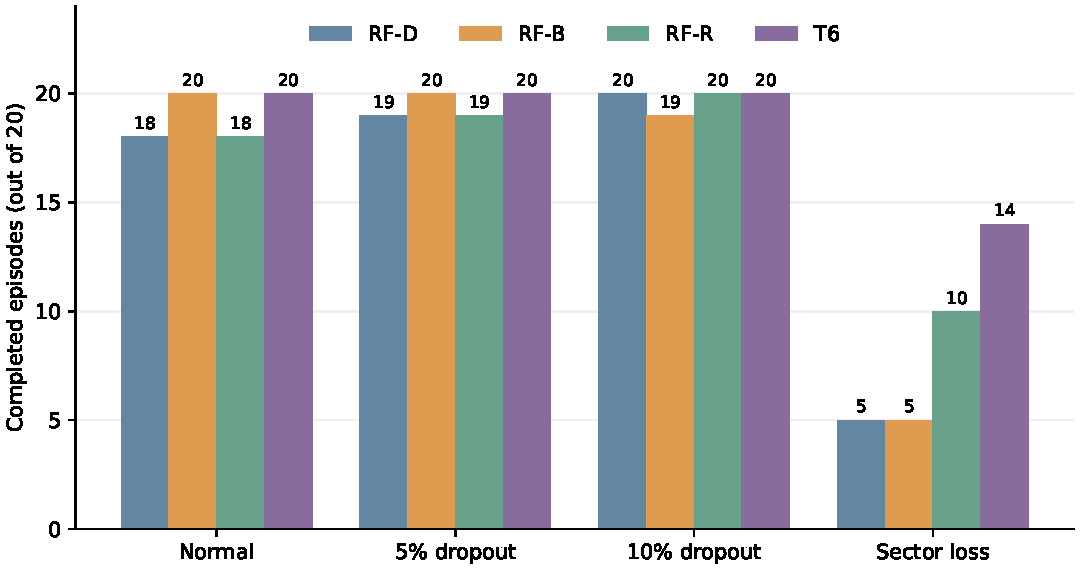
\includegraphics[width=\textwidth]{completion_by_condition.pdf}
\caption[Completion by sensor condition]{Completed episodes out of 20 per sensor condition, computed from
the four primary reports. Each condition aggregates four maps and five starts
per map; bars are descriptive counts, not independent-map reliability estimates.}
\label{fig:completion}
\end{figure}

The strongest offline accuracy belongs to RF-R, whereas the best primary
closed-loop completion count belongs to T6. This mismatch answers the central
comparison question: prediction accuracy alone does not rank these controllers
by their recorded driving outcomes. The student repeatedly selects its own
future observations during driving, whereas the offline data are teacher
trajectories. This distinction is consistent with the learner-induced state
distribution problem in sequential imitation~\cite{ross2011reduction}.
Model-selection decisions should therefore retain the two
levels of evidence rather than replace closed-loop testing with a single
classification score.

\section{Augmentation and Sensor Loss}
RF-B improves on RF-D by two completions in the primary matrix, but RF-R
completes more episodes than either. The observed data do not demonstrate a
consistent advantage from the chosen scattered-dropout augmentation. They
also do not show that augmentation is generally ineffective: the conclusion
concerns this masking rule, this training distribution and these model
configurations.

Forty-six of the 53 primary collision episodes occur in the sector condition.
Scattered loss preserves measurements across much of the visible region,
whereas a contiguous blind region can remove neighbouring directions at the
same time. The recorded outcomes are consistent with sensitivity to this
spatial difference. However, the per-step logs do not contain the original
scan or exact masking indices, so the study cannot identify a particular
missing angular segment as the demonstrated cause of each collision.

The primary matrices also show that an apparently easy map can mask an
important limitation. RF-D and RF-B both complete all five E2 sector episodes
but fail all five on each of the other three maps. Thus E2 sector success
cannot stand alone as evidence of robust operation across the evaluated
geometries.

\section{Repeated Runs and Training Seeds}
A second complete T6 matrix again records 74 completions and six collisions,
with a score of 89.10. An additional sector-only run again completes fourteen
of twenty episodes. RF-R's sector repeat decreases from ten completions to
eight. These repeats indicate both stable patterns and some sensitivity to
repeated execution under nominally matching settings.

Boundary repeats on R1 illustrate why small differences should be interpreted
carefully. RF-D changes from three of five normal completions in its primary
matrix to five of five in the repeat, while its dropout10 result changes from
five of five to three of five. RF-B changes from four to five dropout10
completions. Fixed seeds do not eliminate all runtime variation, but the
available logs do not establish a specific simulator or scan-timing cause.

Additional RF-B models trained with seeds 43 and 44 are evaluated on normal
and sector inputs only. Their normal completions are 20/20 and 19/20,
respectively; both complete 5/20 sector episodes. Seed 42 has 20/20 normal and
5/20 sector completions. These 40-episode subsets are not full 80-episode
matrices. T6 trained with seeds 42, 43 and 44 produces identical exported
headers, so the extra seed artifacts are not counted as three different
deployed tree policies or three new closed-loop experiments.

\section{Cross-Batch Offline Assessment}
The later batch is assessed without changing any fitted model.
Table~\ref{tab:crossbatch} reports equal-map averages across the four maps.
The corresponding project report is identified in Appendix~\ref{sec:evidence_analysis}.
Because three are fitting maps, these averages are not estimates of
unknown-map generalisation. They describe prediction on a later collection
with new starts and a different seed under the same map set.

\begin{table}[htbp]
\centering\small
\caption[Cross-batch offline assessment]{Later-batch offline metrics, averaged equally over four maps.
Macro F1 uses the fixed six-label set and zero for undefined class scores.}
\label{tab:crossbatch}
\begin{tabular}{lrrrr}
\toprule & \multicolumn{2}{c}{Raw} & \multicolumn{2}{c}{Dropout} \\
\cmidrule(lr){2-3}\cmidrule(lr){4-5}
Model & Accuracy & Macro F1 & Accuracy & Macro F1 \\\midrule
RF-D & .8522 & .4204 & .8495 & .4188 \\
RF-B & .8536 & .4210 & .8515 & .4196 \\
RF-R & .8569 & .4203 & .8553 & .4194 \\
T6 & .8530 & .5007 & .8471 & .4869 \\
\bottomrule
\end{tabular}
\end{table}

Under matching aggregation, the archived cross-batch comparison reports small
accuracy and MAE differences for most model/input combinations. This supports
consistency under the observed collection change, not an absence of all
possible distribution shifts. On later-batch E2 raw input, T6 has accuracy
about 0.666, compared with approximately 0.753--0.769 for the forests. Its
fixed-six-class F1 is nevertheless higher. That observation repeats the
metric-ranking distinction seen in the earlier validation.

Later-batch E2 contains thirteen label-5 samples and no label-12 samples.
Fixed-label F1 and present-class F1 therefore need separate interpretation.
Cross-batch changes in a macro score may reflect both predictions and changing
class support. The individual support counts are retained in the accompanying
analysis artifacts instead of attributing every aggregate change to improved
or degraded learning.

\section{Failure Cases and Interpretation}
Figure~\ref{fig:collisionmaps} shows the primary collision endpoints. The seven
non-sector collisions all occur on R1, at approximately 52.6--169.8~s.
Several terminate near similar bends at around 169~s and 33.8~m of travel.
This locates a recurrent difficult region, but does not by itself establish
whether the cause is scan timing, accumulated steering error or a particular
input partition.

\begin{figure}[htbp]
\centering\includegraphics[width=\textwidth]{r6_collision_map.png}
\caption[Collision endpoints on the evaluated maps]{Primary collision endpoints on the four maps, reproduced from the
archived failure analysis. Overlapping markers may represent multiple episodes.
Map coordinates are in metres.}
\label{fig:collisionmaps}
\end{figure}

Successful sector episodes contain more total action switches than early
collision episodes. Since successful episodes run for longer, raw switching
counts are confounded by exposure time. A claim that rapid corrections cause
success would require switching rates or aligned trajectory windows, together
with the relevant observations. The current evidence supports a description
of the action sequences, not this causal explanation.

Likewise, the higher rare-class recall of T6 is a possible contributor to its
behaviour, but the comparison changes several model properties simultaneously.
The appropriate conclusion is that the tested T6 configuration is a stronger
candidate under the current matrix. Isolating depth, feature sampling or
ensemble effects requires additional matched comparisons.

\section{Implications for the Proposed Training Strategy}
The forest results show that teacher-generated supervision can produce useful
LiDAR-only driving without human-labelled trajectories in this pipeline. The
single-tree result shows why the research objective must remain broader than
confirming an initial model preference: a simpler tested student can retain
more useful closed-loop behaviour than the selected shallow ensembles. This
favours further investigation of T6 while preserving the role of the forests
as the principal design candidates and data-variant comparisons.

The result also constrains the automation claim. The teacher's collection
coverage and the student's representation determine which situations are learnt.
Large quantities of cruising data do not automatically cover states caused by
student errors or contiguous sensor loss. Additional automated data should
therefore be directed at a demonstrated gap, with its effects evaluated in
closed loop, rather than assuming that more simulation alone solves the problem.

No matched human-labelled training baseline or physical power measurement is
available. The evidence supports an alternative source of supervision and
candidate compact policies; it does not yet quantify savings in labour or energy.

\section{Limitations and Outstanding Evaluation}
Each map/condition cell has only five starts, and repeated starts on the same
four maps do not establish a broad distribution of environments. Correlated
frames, paired augmentations and identical exported policies must not be
counted as independent replication. Aggregate counts in this chapter are
therefore descriptive; no statistical significance claim is made.

The independent-map and student recovery experiment remains pending. Its
planned base design comprises two frozen models, two new maps, three start
classes and five episodes per cell, giving 60 episodes. A further 40 episodes
would evaluate dropout10 and sector conditions from normal starts on the new
maps. These are proposed measurements, not results. Teacher near-wall
collection cannot fill the missing student-recovery evidence.

Finally, the evaluated policies depend on a fixed forward speed, a limited
action set and a single scan. Wider tasks involving reverse motion, dynamic
obstacles or route planning have not been tested. Host export agreement does
not establish physical timing or safety. These boundaries allow the completed
simulation findings to be used without extending them to unsupported claims.

% !TeX root = ../main.tex
\chapter{Conclusions and Future Work}
\label{ch:conclusions}
\section{Purpose and Completed Contribution}
This project investigates how a digital-twin-oriented training environment can
replace manual driving demonstrations when developing a navigation policy for
a resource-constrained board. The implemented solution assigns different roles
to different models: a PPO-trained neural teacher learns from reward feedback
in a virtual vehicle, while a supervised tree student learns the teacher's
LiDAR-to-action mapping. Training remains a host-side activity and the exported
student is the candidate for eventual onboard inference.

The contribution is the connection between these stages. The virtual platform
provides controlled interaction and privileged state; the teacher supplies
commands without human per-sample action labels; the collector preserves scan
and action pairing; and the student/export workflow produces a separately
evaluable controller. The present evidence covers the virtual training side,
rather than a completed physical twin or a demonstrated low-power deployment.

\section{Answers to the Research Questions}
\textbf{RQ1: Automated supervision.}
The selected PPO--MLP teacher supplies two completed collection batches containing
1,439,983 and 1,079,979 original LiDAR--action pairs, respectively. The collection
process uses teacher commands rather than human driving labels, with model,
map and episode provenance retained. Its separate T3 qualification completes
eight episodes without recorded collision or listed motion failure. These
records establish automated supervision under the implemented conditions.
They do not measure how much operator time is saved or show that teacher labels
are better than human labels. Reward design, modelling and experiment selection
remain engineering responsibilities.

\textbf{RQ2: Transfer to compact policies.}
The automatically generated data support useful student cruising. Across the
normal and scattered-dropout conditions, the forests complete between 57 and
59 of 60 primary episodes and the single tree completes all sixty. Over all
conditions, the forests complete 62--67 of 80 episodes and the single tree
completes 74. Offline action accuracy does not reproduce this closed-loop
ranking. Contiguous sector loss accounts for 46 of the 53 primary collisions,
and the selected scattered-dropout augmentation gives no consistent advantage.
The strongest tested candidate is therefore the single-tree configuration,
although the comparison does not isolate one structural cause. This result
supports the wider objective of obtaining a compact useful policy, while
qualifying the initial choice of a random forest.

\textbf{RQ3: Resource-constrained deployment.}
Tree depth and estimator count make the threshold-evaluation workload explicit,
and the exported C++ implementation agrees with the fitted model on the checked
host inputs. These properties justify pursuing embedded integration. They do
not establish Flash occupancy, peak RAM, worst-case control latency or energy
per decision on the intended board. Nor does successful export establish that
the physical sensor and actuator interfaces reproduce the simulated ones.
The final low-power deployment objective therefore remains partially answered.

\section{Interpretation of the Method Choices}
RL addresses the lack of an initial action-labelled dataset by learning from
sequential outcomes. PPO provides the implemented actor--critic training
procedure, and the MLP represents the teacher's policy and value function.
Privileged geometry is useful because the teacher's immediate role is to
produce demonstrations; the student is subsequently restricted to the sensor
representation available for deployment. A forest offers bounded-depth tree
inference and ensemble aggregation, while the single tree tests whether a
simpler configuration suffices. These choices form a coherent division of
training and deployment responsibilities, not a claim that PPO, MLPs or forests
are individually optimal for every navigation task.

The experimental lesson is that the workflow should be judged by the quality
of the generated supervision and the behaviour and implementation cost of its
student. Selecting a family for practical reasons is a starting hypothesis;
the closed-loop comparison can legitimately favour a different compact member
of the candidate set. The main research purpose is preserved when that happens.

\section{Limitations and Priorities}
The next simulation priority is the frozen-candidate comparison on independent
maps and perturbed student starts. Recovery criteria and observation windows
should be fixed before execution. Selected failure replays with original and
corrupted scans, mask indices and decision timestamps would then help explain
the recurrent R1 and sector collisions. Matched structural comparisons would
be needed before attributing the tree/forest difference to depth or ensembling.

A direct test of the manual-demonstration replacement claim would compare the
automated workflow with a documented human-driven or scripted-teacher baseline
under matched tasks and student settings. Relevant measurements include
operator involvement, collection cost, coverage and resulting driving behaviour.
The absence of that comparison limits claims about efficiency, without changing
the recorded fact that this pipeline generated its action labels automatically.

The later physical phase should calibrate the virtual vehicle against the real
platform, verify sensor/action correspondence, and measure compiled memory,
control latency and energy together with repeated driving outcomes. This would
connect the implemented virtual training side to the intended physical twin and
low-power controller. Until then, the dissertation establishes an automated
simulation-to-student training mechanism and identifies the evidence still
needed for its full embedded objective.


\clearpage
\phantomsection
\addcontentsline{toc}{chapter}{References}
\bibliographystyle{unsrtnat}
\bibliography{references}

\clearpage
\appendix
% !TeX root = ../main.tex
\chapter{Experimental Evidence and Reproducibility}
\label{app:evidence}
\begingroup\raggedright
\section{Source Organisation}
\label{sec:evidence_sources}
Paths are relative to the repository root. The manuscript uses artifacts
available on 31 October 2026, indexed in
\path{article/experiment_data/experiment_index.json}. The R0, R1 and R6 project
reports cover primary runs, cross-batch predictions and failure interpretation.

Teacher provenance is stored under
\path{Gazebo_simulation/rl_models/privileged/policies/validated_privileged_2392588_20261011_074049/}.
The saved configuration and validation summary define the selected teacher's
training and qualification scope. Inspection of the saved policy metadata,
weight dimensions and restored policy verifies the separate actor and critic
MLPs reported in Table~\ref{tab:teacher_network}. The archived training source
identifies PPO with \texttt{MlpPolicy}; the collector uses deterministic teacher
actions. These records distinguish the neural RL teacher from the supervised
forest student. Collection metadata are in
\path{Gazebo_simulation/results/datasets/}, with batch identifiers
\path{collection_20261023_092900_850f9f} and
\path{collection_20261028_141457_3f19f1}. Their training CSV mirrors are under
\path{dataset/simulation/}. The later batch remains outside student fitting.

\section{Model and Report Identification}
\label{sec:evidence_models}
The model directories under \path{software/ML_model/} are
\path{simulation} (RF-D), \path{simulation_both} (RF-B),
\path{simulation_raw} (RF-R) and \path{simulation_tree6} (T6).
Each contains the Python artifact, training report and generated header.
The following identifiers are abbreviated joblib SHA-256 prefixes; full
hashes are recorded in the associated reports and the evidence manifest
stored with this draft.

The manifest also records the header hashes and structural counts underlying
Table~\ref{tab:artifact_resources}. Teacher parameter counts are derived from
Table~\ref{tab:teacher_network}; neither analysis measures compiled board resources.

\begin{table}[htbp]
\centering\small
\caption{Primary model and report mapping.}
\label{tab:sources}
\begin{tabular}{lll}
\toprule Model & Model SHA-256 prefix & Primary report ID \\\midrule
RF-D & \texttt{174279ddbe9d} & \texttt{20261028\_094226\_2350c8} \\
RF-B & \texttt{21939959033b} & \texttt{20261028\_091853\_3d505d} \\
RF-R & \texttt{6974065e6e9b} & \texttt{20261028\_101826\_20b5ff} \\
T6 & \texttt{f8baded18b84} & \texttt{20261028\_121956\_cae76d} \\
\bottomrule
\end{tabular}
\end{table}

The report IDs in Table~\ref{tab:sources} omit the common
\path{evaluation_} prefix. The primary reports are under
\path{Gazebo_simulation/results/random_forest/}. T6's second full run is
\path{evaluation_20261028_125719_d68421}; its separate sector repeat is
\path{evaluation_20261028_124425_3618fe}. RF-R's sector repeat is
\path{evaluation_20261028_104332_15434d}. The seed-43 and seed-44 RF-B subsets
are \path{evaluation_20261028_141057_d342d9} and
\path{evaluation_20261028_142118_c226a4}.

The historical normal report dated 25 October is excluded from the strict
primary comparison because its code-version provenance is insufficient to
establish exact protocol equivalence. Smoke tests verify operation but are
not included in the 320-episode primary matrix.

\section{Analysis Artifacts and Draft Status}
\label{sec:evidence_analysis}
The offline validation tables use the archived cross-evaluation results in
\path{article/experiment_data/C_README.md} and the corresponding model reports.
The later-batch metrics use the R1 report and index. Per-class support,
confusion matrices and per-episode values are retained in the analysis
directory. This draft does not regenerate the million-row offline evaluation.
The primary completion figure is regenerated directly from the four raw
closed-loop JSON reports.

Independent-map recovery (R2), physical trials and target-board measurements
remain future work. The originality, supervisor and authorship statements
are not included in this draft; the applicable institutional declarations
must be completed before submission.

\endgroup

\end{document}
